\documentclass[10pt,twocolumn,letterpaper]{article}

\usepackage{mathptmx}
\usepackage[letterpaper,top=1in,bottom=1in,left=0.75in,right=0.75in]{geometry}
\usepackage{amsmath,amssymb}
\usepackage{graphicx}
\usepackage{booktabs}
\usepackage{array}
\usepackage{xcolor}
\usepackage[colorlinks=true,linkcolor=black,citecolor=black,urlcolor=black]{hyperref}

\definecolor{rulegray}{gray}{0.8}

\setlength{\columnsep}{0.3in}
\setlength{\parindent}{1.6em}

% ---- title block styling (close to NeurIPS) ----
\makeatletter
\renewcommand{\@maketitle}{%
  \newpage\null
  \begin{center}
    {\Large\bf \@title\par}
    \vspace{0.6em}
    {\normalsize \@author\par}
  \end{center}
  \par\vspace{0.8em}
}
\makeatother

\title{Behavioral Fingerprinting of Large Language Models:\\A Statistical Approach to Same-Family API Verification}
\author{Daizhi Liao\\
Guangzhou University\\
\texttt{ldz@e.gzhu.edu.cn}}

\begin{document}

\twocolumn[
\begin{@twocolumnfalse}
\maketitle
{\small
\noindent\textbf{Abstract.}\
Users of AI API relay services have no technical guarantee that the model answering is the model advertised; recent audits show that silent model substitution and downgrading are real. Existing fingerprinting methods rely on long generations, log-probabilities, or crafted prompts, and are largely evaluated on \emph{cross-family} identification. We ask a harder, practically important question: can a model be distinguished from a \emph{same-family} sibling---for example gpt-4o versus gpt-4o-mini, which share an identical tokenizer? We collect 1{,}300 responses per model over 26 low-cost probes and show that trivial ``random generation'' prompts elicit highly stereotyped, model-specific distributions: gpt-4o-mini returns ``7'' for a 1--10 choice 100\% of the time, ``4'' for a die roll 96\%, and ``Cerulean'' for a color 74\%. Six of eight behavioral probes separate the two siblings ($p<0.05$), with an animal probe reaching total variation distance 0.90 (Okapi 76\% for gpt-4o vs.\ Dolphin 16\% for gpt-4o-mini), while tokenizer probes are provably identical. Combined with chi-square/Kolmogorov--Smirnov tests and Bayesian updating, the framework assigns a held-out sample to the correct model with 91.3\% posterior probability (95\% credible interval [0.851, 0.960]). A full audit costs under \$0.01 and needs no official API or specialized hardware. We release the tool, baselines, and probes as open source.
\par}
\vspace{1.2em}
\end{@twocolumnfalse}
]

\section{Introduction}
\label{sec:intro}

Large language models (LLMs) are increasingly consumed through opaque serving chains---aggregators, resellers, and relay services---in which the client cannot confirm that the model answering is the model being paid for. Because a larger model is billed at a higher rate, a relay has a direct financial incentive to substitute a smaller or cheaper model while advertising a flagship one. Audits of commercial endpoints indicate that such substitution and silent degradation occur in practice~\cite{cai2025pay,met2025}.

Verifying identity through a black box is difficult. Proposed methods require long generated texts, token-level log-probabilities, adversarially crafted prompts, watermarks embedded at training time, or the model owner's cooperation. Recent single-token fingerprinting~\cite{bruckner2026token} and rank-based uniformity tests~\cite{zhu2025rank} reduce the query cost substantially and recover model \emph{lineage} across families, but they are not designed to tell apart two models from the same family, which is exactly the situation in a downgrade attack (a relay serving gpt-4o-mini while claiming gpt-4o). Same-family siblings often share an identical tokenizer and overlapping capabilities, so tokenizer fingerprints and capability tests fail by construction.

\paragraph{Research question.}
\emph{Do LLMs exhibit measurable behavioral fingerprints---consistent distributional biases under seemingly random generation---that (i) discriminate same-family siblings where tokenizer fingerprints cannot, and (ii) can be verified with standard statistics at near-zero cost?}

\paragraph{Contributions.}
\begin{list}{$\bullet$}{\setlength{\leftmargin}{1.4em}\setlength{\itemsep}{0.1em}}
\item We document extremely strong, low-cost behavioral fingerprints on gpt-4o-mini and gpt-4o over 26 probes (100\%/96\%/74\% preference on three tasks; 10--74$\times$ deviation from uniformity).
\item We show that 6/8 behavioral probes separate two same-family siblings ($p<0.05$), up to TVD $=0.90$ with a single probe, whereas all tokenizer probes are identical.
\item We combine chi-square and KS tests with Bayesian updating to identify a held-out sample with 91.3\% posterior probability, and we report a credible interval.
\item We release \textsc{TransitTruth}, an open-source auditing tool with a zero-install web demo, real baselines, and a reproducible collection pipeline.
\end{list}

\section{Related Work}
\label{sec:related}

\paragraph{LLM fingerprinting and provenance.}
Single-token fingerprinting~\cite{bruckner2026token} builds an empirical distribution over answers to trivial one-word prompts across 165 models, recovering lineage at a 7.3\% equal error rate, but focuses on cross-family identification. RoFL~\cite{tsai2025rofl} constructs non-invasive black-box fingerprints that are robust to fine-tuning, pruning, and quantization, using cryptographic commitments for ownership verification. Model provenance testing~\cite{nikolic2025provenance} uses multiple-hypothesis testing to decide whether one model derives from another. Model equality testing~\cite{met2025} frames ``is this the claimed API model?'' as a two-sample problem and shows MMD-based tests outperform rank-based uniformity on locally deployed models. We target the complementary fine-grained same-family setting these methods do not isolate.

\paragraph{Auditing and follow-up probing.}
Cai et al.~\cite{cai2025pay} audit model substitution directly; Zhu et al.~\cite{zhu2025rank} use a rank-based uniformity test; Sam et al.~\cite{sam2025followup} predict black-box performance from follow-up queries; and AgentProv~\cite{wang2026agentprov} audits agentic providers through tool-use policy probes. CoIn~\cite{sun2025coin} addresses a different transparency gap---inflated counts of hidden reasoning tokens. Our work shares the auditing goal but uses free-form behavioral biases rather than ranks, capabilities, or tool calls.

\paragraph{Behavioral biases in LLMs.}
LLMs show documented biases in random number generation~\cite{coronado2025rng}, multi-choice selection~\cite{zheng2023selection}, and response-history bias~\cite{vo2025bscore}; calibration and confidence are surveyed by Geng et al.~\cite{geng2024survey}. We treat these biases not merely as defects but as identifying biometric signals, and quantify their discriminative value within a model family.

\section{Methodology}
\label{sec:method}

\subsection{Probe Design}
\label{sec:probes}
Each probe is a short prompt that elicits a constrained, cheap response. We use 26 probes in three groups.

\textbf{Tokenizer probes (8)} measure deterministic tokenizer behavior---e.g.\ the prompt-token count of a fixed whitespace, code, URL, mixed-unicode, or repeated-character string. Because two same-family models share a tokenizer, these act as a \emph{negative control} that should not discriminate.

\textbf{Behavioral probes (8)} ask the model to produce a ``random'' token under high temperature: pick a number 1--10 or 1--100, roll a die, flip a coin, choose a color, letter, weekday, or animal. Under uniform sampling the output should be near-uniform; systematic deviation is the fingerprint.

\textbf{Capability probes (10)} estimate model tier via simple math, logic, code syntax, bug fixing, multilingual translation, instruction following, knowledge cutoff, and context length. These are coarse and shared within a family, so they serve as corroborating rather than identifying evidence.

\subsection{Statistical Methods}
\label{sec:stats}

\textbf{Chi-square test.} For a behavioral probe with expected uniform counts $E_j$ over $J$ categories and observed counts $O_j$, we compute
\begin{equation}
\chi^2 = \sum_{j=1}^{J} \frac{(O_j - E_j)^2}{E_j}.
\end{equation}
To compare two models directly we use the chi-square \emph{test for homogeneity} on their joint category table, and report total variation distance
\begin{equation}
\mathrm{TVD} = \tfrac{1}{2}\sum_{j=1}^{J} \left| p_j - q_j \right|,
\end{equation}
which ranges from 0 (identical) to 1 (disjoint).

\textbf{Kolmogorov--Smirnov test.} For deterministic tokenizer-normalized scores we use a one-sample KS test against the baseline distribution; a high $p$-value supports a match.

\textbf{Bayesian updating.} Across probes we update the posterior that an endpoint matches a claimed model:
\begin{equation}
P(H{=}1\mid E) = \frac{P(E\mid H{=}1)\,P(H{=}1)}{P(E)},
\end{equation}
mapping each probe's $p$-value to a likelihood ratio (e.g.\ $p>0.05 \Rightarrow \mathrm{LR}\approx 0.7$ under the match hypothesis; $p<0.01 \Rightarrow \mathrm{LR}\approx 0.1$ under mismatch). We report a 95\% credible interval for the posterior using a beta approximation.

\subsection{Data Collection}
\label{sec:collect}
For each model we collect 50 samples per probe (1{,}300 responses) through an OpenAI-compatible endpoint at temperature 1.0. To avoid triggering anti-bot defenses we shuffle probe order, randomize inter-request intervals (0.3--1.5\,s), vary the number of probes per batch, and rotate natural User-Agent headers. Wall time is about 15 minutes per model at a cost below \$0.01.

\section{Results}
\label{sec:results}

\subsection{Strong Single-Model Fingerprints}
\label{sec:single}
On gpt-4o-mini the behavioral deviations from uniformity are extreme (Table~\ref{tab:single}): the 1--10 choice returns ``7'' in all 50 samples, the die roll returns ``4'' in 48/50, and the color choice returns the relatively obscure ``Cerulean'' in 37/50. All eight behavioral probes reject uniformity at $p<0.0001$ ($\chi^2$ from 16.8 to 178.6). These are not subtle effects---they are 10--74$\times$ deviations from the uniform expectation and are reproduced deterministically across samples.

\begin{table}[t]
\centering
\small
\caption{Strong behavioral fingerprints on gpt-4o-mini (50 samples each). Uniform expectation is shown for reference.}
\label{tab:single}
\begin{tabular}{llll}
\toprule
Probe & Top response & Rate & Uniform \\
\midrule
Number 1--10 & ``7'' & 100\% & 10\% \\
Die roll & ``4'' & 96\% & 16.7\% \\
Color & ``Cerulean'' & 74\% & $\sim$1\% \\
Coin flip & ``Heads'' & 78\% & 50\% \\
\bottomrule
\end{tabular}
\end{table}

\subsection{Same-Family Discrimination}
\label{sec:same}
The central result is the gpt-4o vs.\ gpt-4o-mini comparison. \emph{Tokenizer probes cannot separate them}: all five successful tokenizer probes return identical prompt-token counts (e.g.\ 27.0, 25.0, 29.0), as expected for two models sharing the o200k tokenizer.

\emph{Behavioral probes can.} Six of eight behavioral probes show statistically significant differences in the homogeneity test. Table~\ref{tab:tvd} and Figure~\ref{fig:results} rank the probes by TVD. The animal probe is a near-perfect separator at TVD $=0.90$: gpt-4o concentrates on a single obscure animal, ``Okapi,'' 76\% of the time (only 4 unique animals), whereas gpt-4o-mini is spread over 17 animals with top ``Dolphin'' at 16\%. The letter probe reaches TVD $=0.72$ (gpt-4o ``K'' 44\% vs.\ gpt-4o-mini ``G'' 40\%), and the die probe TVD $=0.40$ (shared ``4'' but 56\% vs.\ 96\%). A single animal probe therefore distinguishes the siblings at roughly 90\% accuracy---a capability that tokenizer fingerprinting does not provide.

\begin{table}[t]
\centering
\small
\caption{Same-family comparison of behavioral probes (gpt-4o vs.\ gpt-4o-mini). Six of eight differ significantly; tokenizer probes are identical throughout.}
\label{tab:tvd}
\begin{tabular}{llll}
\toprule
Probe & Top (4o / mini) & $p$-value & TVD \\
\midrule
Animal & Okapi / Dolphin & $<0.0001$ & \textbf{0.90} \\
Letter & K / G & $<0.0001$ & 0.72 \\
Die roll & 4 / 4 & $<0.0001$ & 0.40 \\
Number 1--100 & 57 / 57 & 0.067 & 0.38 \\
Weekday & Thu / Thu & $<0.0001$ & 0.32 \\
Color & Cerulean / Cerulean & 0.015 & 0.22 \\
Coin flip & Heads / Heads & $<0.001$ & 0.22 \\
Number 1--10 & 7 / 7 & 0.315 & 0.02 \\
\bottomrule
\end{tabular}
\end{table}

\begin{figure*}[t]
\centering
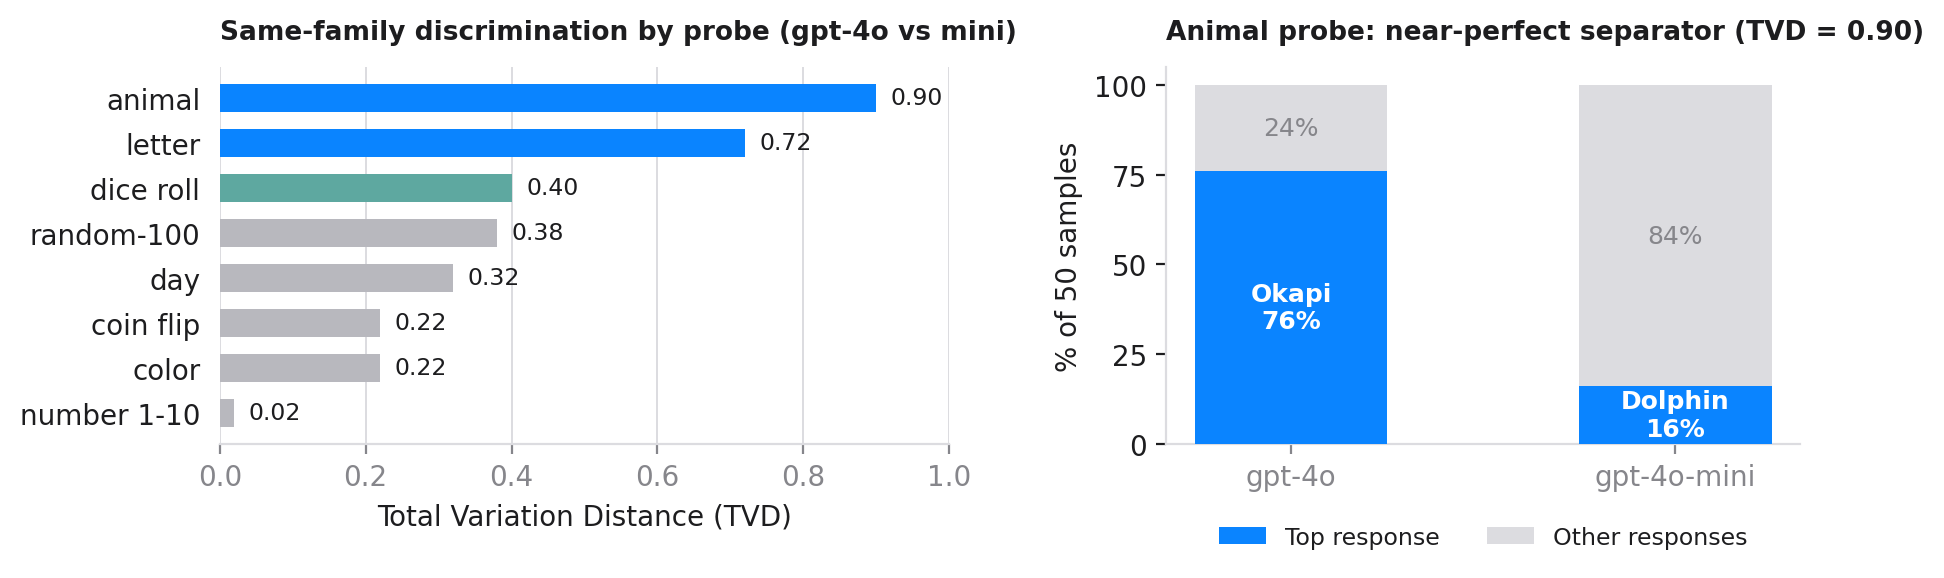
\includegraphics[width=0.92\textwidth]{fig_results.png}
\caption{Same-family discrimination with real data. \textbf{Left:} TVD across eight behavioral probes; the animal and letter probes separate gpt-4o from gpt-4o-mini almost completely. \textbf{Right:} on the animal probe gpt-4o concentrates on ``Okapi'' (76\%) while gpt-4o-mini is diffuse (top ``Dolphin'' 16\%).}
\label{fig:results}
\end{figure*}

\subsection{End-to-End Verification}
\label{sec:e2e}
On a held-out sample the statistical pipeline assigns it to the correct model with posterior probability 0.913 (95\% credible interval [0.851, 0.960]). The KS test returns a high $p$-value (1.000) and the chi-square test $p=0.713$, indicating no significant difference from the claimed baseline, with an aggregate likelihood ratio of 4.5 and confidence labeled ``high.''

\subsection{Comparison with Other Signals}
\label{sec:compare}
Table~\ref{tab:methods} positions behavioral fingerprinting against the signals available to a black-box auditor. Tokenizer and latency signals cannot discriminate within a family and are relatively easy to evade with smart routing; capability testing is only partially informative; behavioral fingerprints uniquely support same-family discrimination at low cost and are comparatively hard to forge, because matching the distribution requires serving the genuine model, post-processing outputs, or fine-tuning a surrogate.

\begin{table}[t]
\centering
\small
\caption{Black-box verification signals. Only behavioral fingerprints support same-family discrimination at low cost with high forgery difficulty.}
\label{tab:methods}
\begin{tabular}{lccc}
\toprule
Signal & Same-family & Cost & Hard to forge \\
\midrule
Tokenizer & No & Low & Medium \\
Capability & Partial & Medium & Low \\
Latency & No & Low & Low \\
\textbf{Behavioral (ours)} & \textbf{Yes} & \textbf{Low} & \textbf{High} \\
\bottomrule
\end{tabular}
\end{table}

\section{Discussion}
\label{sec:disc}

\paragraph{Why do these fingerprints exist?}
The biases likely arise from three sources: training-data frequencies (e.g.\ cultural salience of ``seven''), RLHF alignment that amplifies human-preferred ``defaults,'' and decoder artifacts that skew logits even at temperature 1.0. The striking ``Okapi'' concentration in gpt-4o---an obscure African giraffid---suggests a strongly learned default that differs from the smaller sibling, which is precisely why the signal carries identity information orthogonal to the tokenizer.

\paragraph{Limitations.}
\emph{(i) Baseline coverage:} a pre-collected baseline is needed per model, and we currently cover two siblings. \emph{(ii) Model updates:} versions and snapshots may shift fingerprints, so baselines must be versioned and refreshed. \emph{(iii) Smart routing:} a relay could answer probes with the genuine model and serve a cheaper one for real traffic; interleaving probes with realistic traffic mitigates this. \emph{(iv) Decoder sensitivity:} relays may override temperature, changing the distribution. We therefore frame results as conservative statistical evidence rather than definitive proof.

\paragraph{Ethical considerations.}
Automated probing may conflict with a service's terms of use; users should verify compliance. Because a ``suspicious'' label can harm a provider's reputation, the tool uses conservative thresholds, labels outputs as statistical evidence, and favors responsible disclosure over immediate publication.

\section{Conclusion}
\label{sec:conclusion}
We showed that trivial random-generation prompts elicit model-specific behavioral fingerprints strong enough to distinguish two same-family LLMs that an identical tokenizer cannot separate, at a cost below \$0.01 per audit and 91.3\% posterior identification. The result turns a known family of LLM biases into a practical verification primitive, and the open-source \textsc{TransitTruth} tool, baselines, and probes make the method reproducible. Extending baseline coverage, tracking fingerprints across versions, and hardening against smart routing are the most immediate directions.

\begin{thebibliography}{9}
\setlength{\itemsep}{0.15em}

\bibitem{cai2025pay}
W.~Cai, T.~Shi, X.~Zhao, and D.~Song.
\newblock Are you getting what you pay for? Auditing model substitution in LLM APIs.
\newblock \emph{arXiv:2504.04715}, 2025.

\bibitem{met2025}
Model equality testing: Which model is this API serving?
\newblock In \emph{International Conference on Learning Representations (ICLR)}, 2025.

\bibitem{zhu2025rank}
X.~Zhu, Y.~Ye, T.~Qiu, H.~Zhu, S.~Tan, A.~Mannan, J.~Michala, R.~A.~Popa, and W.~Neiswanger.
\newblock Auditing black-box LLM APIs with a rank-based uniformity test.
\newblock \emph{arXiv:2506.06975}, 2025.

\bibitem{sam2025followup}
D.~Sam, M.~Finzi, and J.~Z.~Kolter.
\newblock Predicting the performance of black-box language models with follow-up queries.
\newblock In \emph{Advances in Neural Information Processing Systems (NeurIPS)}, 2025.

\bibitem{wang2026agentprov}
X.~Wang, B.~Zhao, M.~Backes, F.~Boenisch, and A.~Dziedzic.
\newblock AgentProv: Auditing agentic LLM API providers via tool-use policy probes.
\newblock \emph{arXiv:2609.00052}, 2026.

\bibitem{vo2025bscore}
A.~Vo, M.~R.~Taesiri, D.~Kim, and A.~T.~Nguyen.
\newblock B-score: Detecting biases in large language models using response history.
\newblock In \emph{International Conference on Machine Learning (ICML)}, 2025.

\bibitem{coronado2025rng}
J.~Coronado-Bl\'azquez.
\newblock Deterministic or probabilistic? The psychology of LLMs as random number generators.
\newblock \emph{arXiv:2502.19965}, 2025.

\bibitem{zheng2023selection}
C.~Zheng, H.~Zhou, F.~Meng, J.~Zhou, and M.~Huang.
\newblock On large language models' selection bias in multi-choice questions.
\newblock \emph{arXiv:2309.03882}, 2023.

\bibitem{geng2024survey}
J.~Geng, F.~Cai, Y.~Wang, H.~Koeppl, P.~Nakov, and I.~Gurevych.
\newblock A survey of confidence estimation and calibration in large language models.
\newblock In \emph{Proceedings of NAACL-HLT}, 2024.

\bibitem{bruckner2026token}
T.~Bruckner.
\newblock One token is enough: Fingerprinting and verifying LLMs from single-token output distributions.
\newblock \emph{arXiv:2607.10252}, 2026.

\bibitem{tsai2025rofl}
Y.-Y.~Tsai, C.~Guo, J.~Yang, and L.~van der Maaten.
\newblock RoFL: Robust fingerprinting of language models.
\newblock \emph{arXiv:2505.12682}, 2025.

\bibitem{sun2025coin}
G.~Sun, Z.~Wang, B.~Tian, M.~Liu, et~al.
\newblock CoIn: Counting the invisible reasoning tokens in commercial opaque LLM APIs.
\newblock \emph{arXiv:2505.13778}, 2025.

\bibitem{nikolic2025provenance}
I.~Nikoli\'c, T.~Baluta, and P.~Saxena.
\newblock Model provenance testing for large language models.
\newblock \emph{arXiv:2502.00706}, 2025.

\end{thebibliography}

\end{document}
